\chapter{Improvements of Ecotype Simulation}

%\begin{shadequote}
%\begin{center}
%    \Large\begin{verbatim} 
%        Harder, Better, Faster, Stronger
% \end{verbatim}  
%\end{center}
%\par--\emph{Daft Punk}
%\end{shadequote}

\begin{shadequote}
\begin{center}
    \Large\begin{verbatim} 
             Citius, Altius, Fortius
 \end{verbatim}  
\end{center}
\par--\emph{Olympic Motto}
\end{shadequote}
%%Faster, Higher, Stronger


\section{Improvements}
ES1 set hard input size limits of 2000 sample sequences of at most 3000 nucleotides~\cite{koeppel2008identifying}.
However, I doubt it was ever run with even close to that many sequences.
When run on input sizes of greater than only one hundred sequences time became a limiting factor.
In fact previous work showed that while ES1 had superior demarcation accuracy to its contemporaries, ES1 could not compete in run-time comparisons.
And as we increase the sample size running time increases dramatically.
See Table \ref{tab:ES1speed}.
This issue is clearly a priority for improvement.

To solve the problem we came up with two approaches.
First, modify the main ES algorithm driving the program.
Second, reorganize execution to take advantage of large computer clusters (parallelization).
I will focus mainly on modifications to the ES algorithm, which are prominently featured in ES2, and briefly address my colleague, Lingyuan Ke's, approach to (parallelization) which will be featured in future Ecotype Simulation iterations.
Finally, I will discuss future plans for improving the Ecotype Simulation software family.


\subsection*{Ecotype Simulation 2.0}
This is the version of ES I thoroughly test in chapter chapter four in comparison to other demarcating programs.
While the changes are few in number, we believe that they will increase the practicality of using ES approach to understanding microbial diversity.

\begin{table}
 %\begin{tabular}{| l | l | l | l |}
 \begin{tabular}{| c | c | c | c |}
  \hline
  Algorithm & 20 sequences & 30 sequences & 50 sequences \\ \hline
  ES & 69.8 & 384 & 2390 \\
  AdaptML & 1.54 & 1.57 & 1.64 \\
  GMYC & 0.201 & 0.292 & 0.549 \\
  BAPS & 4.80 & 5.15 & 6.12 \\
  \hline
 \end{tabular}
 \caption[ES1 run-time compared to other demarcation programs.]{The run speed is measured in seconds (reprinted from \protect\cite{carlo})}
 \label{tab:ES1speed}
\end{table}

\subsubsection*{Key algorithmic changes}
Backwards and forward simulation takes up most of ES1 run time.
The simulation process is called many times throughout the entire typical program execution.
If we can come up with a way to reduce the time complexity of simulations, great speed improvements are possible.

For ES2 we run the backwards simulation of node coalescence exactly the same.
However, once we have the evolutionary history scaffold we can use properties of ultra-metric phylogenetic trees.
Ultra-metric trees have the same distance between root to tip for all organisms, and usually are made under the assumptions of a molecular clock.
By the length between two nodes we can determine time between organisms.
Based on this fact performing binning is unnecessary.
ES2 can conduct a linear pass through the backwards scaffold directly comparing it to the observed sequence identity graph, checking for success and failure with all precision levels.
This insight removes an $O(n^3)$ factor, immediately quickening the algorithm.

\subsubsection*{Demarcation}
In addition to core algorithm changes we made changes to the auto-demarcating program.
Instead of demarcation confidence intervals, ES2 runs the downhill-simplex (Hillclimbing) method on each subtree as we recursively descend through the phylogeny.
Normally our Bruteforce method must be run before Hillclimbing, in this case we use results from Hillclimbing as a seed for the closest ancestor node.
Then at each child node we use Hillclimbing results from the parent node, bypassing running Bruteforce for each subtree.
This maintains a high level of accuracy without compromising speed.

%THINK ABOUT HOW TO ORDER THIS SECTION AND MAKE HEADERS
\section{Future Improvements}
Through the work involved with this project we realized that in addition to speed, space has become a limiting factor.
To make a distance divergence matrix we need $O(n^2)$ space, and with sequence sizes in the thousands we very quickly run out of RAM. Also, the current implementation has similar time complexity to the naive $O(n^3)$ approach.
We explored different clustering packages that had various space and time trade-off balances.

Besides improving our clustering technique, parallelizing the ES algorithm is the highest priority.
I will briefly overview our designs and results in parallelizing ES.
However, the reader should refer to, my colleague, Lingyuan Ke's senior thesis for full details.
%\subsection*{Ecotype Simulation 3.0}
\subsection*{Binning}
As mentioned in previous sections ES uses complete linkage clustering.
The current implementation is in Fortran90, and we have yet to update it to reflect improvements in the state of the art.
Big Data companies have developed an interest in clustering large datasets, resulting in various improvements in clustering algorithms.
\subsubsection*{Current implementation}
%First I'll go over our naive implementation here
Our naive approach is as follows:
%FROM WIKIPEDIA!  CITE!
\begin{enumerate}[I]
\item Begin with the disjoint clustering having level $L(0) = 0$ and sequence number $m = 0$.
\item Find the most similar pair of clusters in the current clustering, say pair $(r)$, $(s)$, according to $d[(r),(s)] = max$ $d[(i),(j)]$ where the maximum is over all pairs of clusters in the current clustering.
\item Increment the sequence number: $m = m + 1$. Merge clusters $(r)$ and $(s)$ into a single cluster to form the next clustering m. Set the level of this clustering to $L(m) = d[(r),(s)]$
\item Update the proximity matrix, $D$, by deleting the rows and columns corresponding to clusters $(r)$ and $(s)$ and adding a row and column corresponding to the newly formed cluster. The proximity between the new cluster, denoted $(r,s)$ and old cluster $(k)$ is defined as $d[(k), (r,s)] = max$ $d[(k),(r)]$, $d[(k),(s)]$.
\item If all objects are in one cluster, stop. Else, go to step II.
\end{enumerate}
which ends up running at $O(n^3)$ time (written up using~\cite{wiki:xxx} as a reference).
In our case we divide the processing by first calculating a pairwise distance matrix between all sequences.
That way we maintain a look up table, $D$, to look up distance in constant time.
At each iteration two clusters are merged (specifically the closest by the specified distance function) and the divergence matrix is updated with a distance entry between each cluster and the new cluster (specifically the element of each cluster being compared that is the farthest apart).

\subsubsection*{State of the art}
From the literature we discovered that there are complete-linkage clustering implementation that achieve $O(n^2)$ time complexity.
We found fastcluster, a well-documented and tested C++ library that efficiently implements several a hierarchical clustering algorithms~\cite{mullner2011modern, FastClust}.
The library includes complete-linkage clustering that runs in $O(n^2)$ (for a graphical comparison of various clustering package see Figure~\ref{fig:FastClustComparison}).

\begin{figure}[h!]
\centering
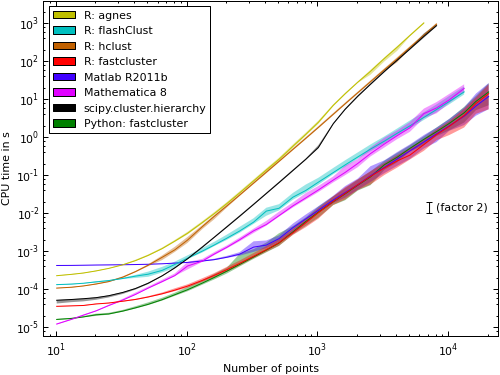
\includegraphics[scale=0.7]{images/FastComplete-CH3}
\caption[Complete linkage clustering speed comparison between popular implementations.]{The colored bands show maximum and minimum time over a variety of data sets. The average is plotted as a solid line. The synthetic data sets are samples drawn in an iid. manner from various mixtures of Gaussian distributions in Euclidean space of various dimensions.
%The results were obtained on a PC with an Intel dual-core CPU T7500 with 2.2 GHz clock speed and 4GB of RAM. The operating system was Ubuntu 11.04 64-bit (Ubuntu 10.04 64-bit for Matlab R2010a). R version: 2.13.0, fastcluster version: 1.1.7, flashClust version: 1.01, Python version: 2.7.1, NumPy version 1.5.1, SciPy version: 0.8.0.
(reprinted from \protect\cite{FastClust})}
\label{fig:FastClustComparison}
\end{figure}

I quickly linked up fastcluster to ES2, replacing our naive binning implementation and was achieving impressive speed results. However, we are not enthusiastic about adding another dependency to ES2. For now it's a envisioned improvement for the next version of ES.

%Include excel picture of comparison!


\subsubsection*{Minimizing space usage}
%None of that matters if we can't decrease the space usage.
%Approach one, don't save a divergence matrix
%Here I could include some of my code.
While
%Approach two, bin in parallel.

\subsection*{Parallelization}
%Talk a little bit about the parallelization plans we have. Hybrid mp and mph
%and how it'll be the next step in the ES evolution
\subsubsection*{OpenMP approach} %WIKI EXACT OPERATION OF OPENMP!!!
The OpenMP API is a commonly used shared-memory parallelism approach designed for C, C++, and Fortran programs.
In Fortran the programmer adds comments (known as directives) to specify OpenMP behavior.
These directives implicitly or explicitly define, perhaps guide, the execution of multiple threads as parallel programs

An OpenMP enriched program begins as a single thread of execution.
Whenever a thread encounters a parallel construct the thread creates a team of sub-threads, generates a set of tasks, and then declares itself master of the team.
Only the master thread resumes execution beyond the end of the parallel construct.
The program can specify any number of parallel constructs.

All threads have access to the same memory so they can retrieve variables, this is called a shared-memory model.
Also, each thread can specify private memory unreachable to other threads.
We use shared and private clause keywords to identify the respective paradigm.
%HERE LING REFERENCES AN ARTICLE

\subsubsection*{Tests}
%Outline best results from Ling's tests
